\chapter{Microservices en monolieten}
\label{ch:microservices}

De meeste programma's worden gemaakt door een monolothische architectuur te hanteren (\cite{villamizar_evaluating_2015}). Alle functionaliteit en verantwoordelijkheden worden gestopt in één programma. Dit soort van programma wordt een monoliet of monolith in het Engels genoemd. De architectuur waarin deze soort programma's voorkomen noemen we een monolithische architectuur. Software ontwikkelaars structureren door middel van patronen (\cite{tichy_catalogue_1997}) om functionaliteit en verantwoordelijkheid van elkaar te scheiden. Modulariteit is hierbij een belangrijk gegeven.

\begin{wrapfigure}{r}{0.4\textwidth}
    \centering
    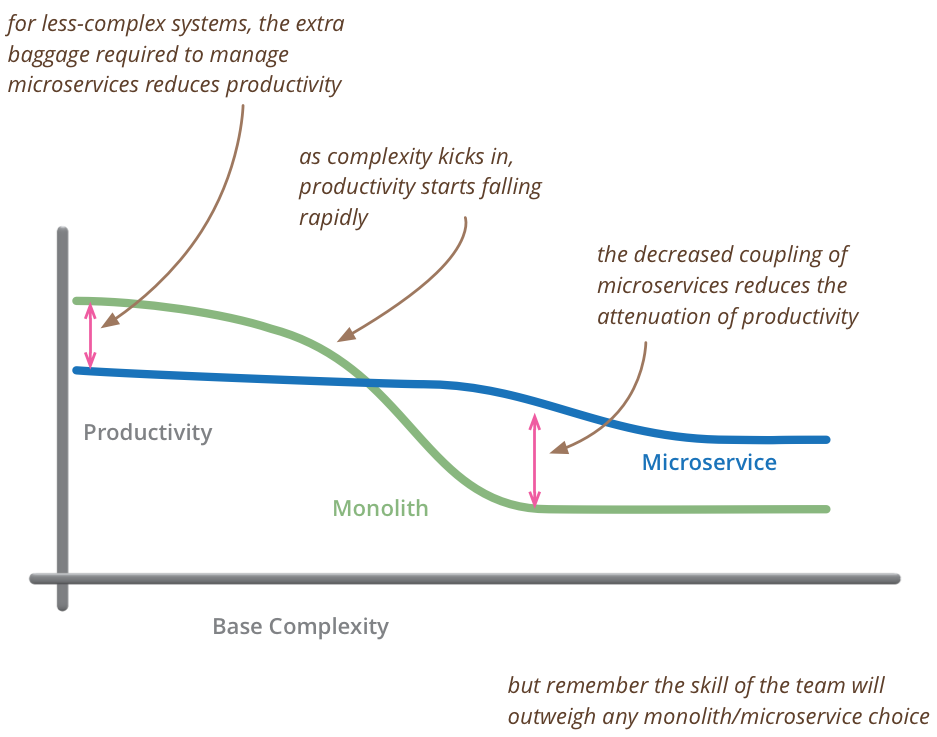
\includegraphics[width=6cm]{img/microservices_monolith}
    \caption[Vergelijking microservices en monolieten]{Productiviteit en complexiteit van microservices architectuur tegenover een monolithische architectuur (\cite{martin_fowler_microservicepremium_2015})}
    \label{fig:pr}
\end{wrapfigure}

Een probleem dat veel voorkomt bij een monolithische architectuur is dat het programma zeer complex wordt na verloop van tijd (\cite{villamizar_evaluating_2015}). Functionaliteit toevoegen is niet vanzelfsprekend bij een complex programma, want er moet rekening worden gehouden met de andere delen van het programma. Nieuwe software ontwikkelaars die het programma niet kennen moeten eerst een paar weken het programma verkennen. Dan pas kan er begonnen worden met nieuwe functionaliteit te schrijven.

Schaalbaarheid is een probleem waar ook tegen gelopen wordt na verloop van tijd (\cite{villamizar_evaluating_2015}). Sommige onderdelen van een programma moeten meer trafiek kunnen verwerken dan andere delen. Zoals al aangehaald werd in hoofdstuk \ref{ch:virtualisatie}, hebben verschillende soorten programma's andere middelen nodig. Dit is hetzelfde bij de interne delen van programma. Het schalen van deze componenten is alleen mogelijk door een nieuwe instantie toe te voegen van de hele applicatie of de implementatie te verbeteren. Eén groot programma is ook niet handig voor grote teams te laten samenwerken. Het uitbrengen van een versie moet dan nagegaan worden bij alle teams die aan dat programma werken.

Al langer bestaat het idee om een groot programma op te splitsen in kleinere programma's. Telecommunicatie is een industrie waarbinnen microservices al werden gebruikt \cite{griffin_survey_2007}. De opkomst van software containers heeft dit deze werkwijze meer verspreid. Dit komt omdat het gemakkelijker is geworden om kleinere programma's met elkaar te verbinden, zelf als ze zich niet op dezelfde omgeving bevinden. De architectuur waarbinnen dit idee wordt gebruikt, wordt microservices architectuur genoemd. De microservices kunnen we bekijken als deelapplicaties die één verantwoordelijkheid hebben.

\begin{wrapfigure}{r}{0.4\textwidth}
    \centering
    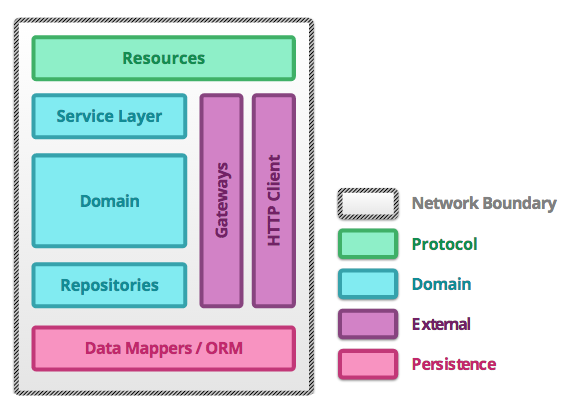
\includegraphics[width=6cm]{img/microservice_structure_example}
    \caption[Structuur architectuur microservices]{Structuur van een architectuur met microservices (\cite{toby_clemson_testing_2014}) }
    \label{fig:microservice_structure_example}
\end{wrapfigure}


Een programma opsplitsen in componenten, met één verantwoordelijkheid, zorgt ervoor dat het meer schaalbaar is. Containers en unikernels helpen hierbij. Het opstarten van een nieuwe instantie van een microservice neemt minder tijd in beslag dan het opstarten van een nieuwe instantie van een monoliet.

Bij microservices zal de topologie van het probleemdomein goed gekend moeten zijn. Starten met het gebruiken van microservices architecture wanneer men het domein niet goed kent, vraagt om problemen. Het ontwerpen van een microservices architectuur moet goed gebeuren. Anders kunnen er problemen voorkomen met impact op de gehele architectuur, bijgevolg moeten er grote delen worden herschreven. Een monolitische architecture zal beter kunnen reageren op dit probleem. Als men later het domein kent kan een microservices architecture worden gebruikt. Hiervoor moet de monoliet modulair geschreven worden. Modulariteit is een vanzelfsprekende bouwsteen binnen programmeren.

De complexiteit van een monoliet wordt overgebracht naar het communiceren en het behouden van de consistentie tussen de microservices. Verder wordt ook het opstellen van de architectuur moeilijker.

Het voordeel van een microservices architectuur is dat de microservices van elkaar gescheiden zijn. Het gebruik van een nieuwe technologie of framework is niet langer een groot probleem. Dit komt omdat de microservices los van elkaar staan. Er kan dus een andere programmeertaal gebruikt worden zolang de communicatie tussen de microservices consistent blijft.

De communicatie van de microservices gebeurd via het netwerk. Dit maakt het mogelijk om microservices op verschillende virtuele machines of software containers te laten werken. Software defined network (\cite{garcia_villalba_trends_2015}) neemt veel complexiteit weg van de communicatie.

\begin{wrapfigure}{r}{0.4\textwidth}
    \centering
    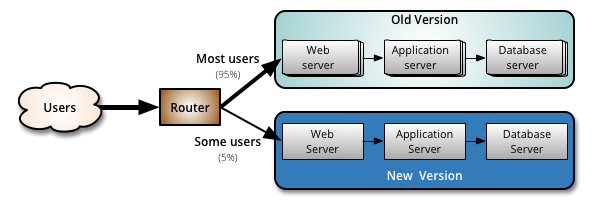
\includegraphics[width=6cm]{img/canary-release}
    \caption[canary release]{Voorbeeld van een canary release (\cite{danilo_sato_canaryrelease_2014})}
    \label{fig:canary-release}
\end{wrapfigure}

Een monolitische architectuur opstellen in productie is relatief simpel tegenover een microservices architectuur. Wanneer er een nieuwe versie moet worden opgesteld in productie kan gebruik worden gemaakt van blue-green deployment (\cite{martin_fowler_bluegreendeployment_2016}). Waarbij we een oude en nieuwe versie hebben van de architectuur en de router het verkeer verlegt naar de nieuwe architectuur. Dit zorgt voor een gemakkelijke overgang.

Bij microservices kan gebruik gemaakt worden van een canary release strategie (\cite{danilo_sato_canaryrelease_2014}). Hier wordt weer een nieuwe versie opgesteld met de laatste veranderingen van de architectuur. De router gaat een deel van het verkeer naar de nieuwe architectuur versturen. Naarmate de tijd vordert, wordt het vertrouwen in de nieuwe versie nagegaan. Als het vertrouwen is toegenomen dan zal meer verkeer naar de nieuwe versie worden gestuurd. Zo kunnen er problemen worden nagegaan en er gepast op reageren. Uiteindelijk krijgt de oude versie geen verkeer meer en wordt alleen de nieuwe versie gebruikt.

De systeembeheerder krijgt meer werk omdat er nu tientallen microservices moeten beheerd worden in plaats van één grote applicatie. Het beheren van deze microservices en hun logs wordt een belangrijke bron van informatie binnen de architectuur. Er kan gezegd worden dat deze microservices simpeler zijn om te verstaan, omdat de functionaliteit per microservices beperkt is. Sommige halen aan dat het de complexiteit die we niet meer tegenkomen in de applicatie nu terechtkomt bij het samen te laten werken van de verschillende onderdelen.